\documentclass[12pt]{article}
\usepackage{latexblog}

% ============================================================
% Blog Metadata
% ============================================================
\blogtitle{B-Tree算法}
\blogdate{2018-12-18}
\blogtags{刨根问底, 算法}
\bloglang{zh}
\blogsummary{}

\begin{document}
\makeblogtitle

B-Tree(区别于二叉树)是一种平衡多叉搜索树。

\section{B-Tree的定义}\label{b-treeux7684ux5b9aux4e49}

根据Knuth的定义，\({\displaystyle m}\)阶的B-Tree有如下的特性：

\begin{enumerate}
\tightlist
\item
  节点左边的元素都比它小，节点右边的元素都比它大
\item
  每个节点最多有\({\displaystyle m}\)个子节点
\item
  除了根节点之外，非叶节点（没有孩子的节点）至少有\({\displaystyle m/2}\)个子节点
\item
  如果根节点不是叶子节点则其至少有两个子节点
\item
  包含\({\displaystyle k}\)个子节点的节点共有\({\displaystyle k-1}\)个键
\item
  所有的叶子节点的高度相同
\end{enumerate}

一般表示B-Tree有两种表示方法：

\begin{itemize}
\tightlist
\item
  B-Tree of order \({\displaystyle d}\) or \({\displaystyle M}\)
\item
  B-Tree of degree or \({\displaystyle t}\)
\end{itemize}

\subsection{\texorpdfstring{Kuath: B-Tree of Order \({\displaystyle d}\)}{Kuath: B-Tree of Order \{\textbackslash displaystyle d\}}}\label{kuath-b-tree-of-order-displaystyle-d}

其中\({\displaystyle M=5}\) 表示每一个节点中\emph{至多有5个子节点}；则有如下的特性：
\begin{align}
&Max(children) = 5 \\
&Min(children) = ceil(M/2) = 3 \\
&Max(keys) = Max(children) - 1 = 4 \\
&Min(keys) = Min(children) - 1 = 2
\end{align}

\subsection{\texorpdfstring{CLRS: B-Tree of min degree \({\displaystyle t}\)}{CLRS: B-Tree of min degree \{\textbackslash displaystyle t\}}}\label{clrs-b-tree-of-min-degree-displaystyle-t}

而\({\displaystyle t=5}\) 则定义了一个节点中\emph{至少有5个子节点}
\begin{align}
&Max(children) = 2t = 10 \\
&Min(children) = t = 5 \\
&Max(keys) = 2t -1 = 9 \\
&Min(keys) = t - 1 = 4
\end{align}

这里degree指的是一个节点中子节点的数目。CLRS中用的最小度，即节点中最少有多少个子节点。例如t=2即表示的是2-3-4 tree，每个子节点中可以有2、3或者4个children。

\subsection{CS673: B-tree of maximum degree k}\label{cs673-b-tree-of-maximum-degree-k}

而也有使用Max degree的，例如\href{https://www.cs.usfca.edu/~galles/visualization/BTree.html}{DB Virtualization}里面，使用的就是最大度（即最多有k个子节点），则：

\begin{itemize}
\tightlist
\item
  所有的interior node最少有k/2个children，最多有k个
\item
  2-3树即对应到maximum degree of 3
\end{itemize}

\subsection{对应关系}\label{ux5bf9ux5e94ux5173ux7cfb}

这些表示方法的对应关系如下：

{\def\LTcaptype{none} % do not increment counter
\begin{longtable}[]{@{}llll@{}}
\toprule\noalign{}
Kunth Order, k & CLRS min degree & CS673 max defree & (min, max) children \\
\midrule\noalign{}
\endhead
\bottomrule\noalign{}
\endlastfoot
k=0 & - & - & - \\
k=1 & - & - & - \\
k=2 & - & - & - \\
k=3 & - & t=3 & (2, 3) \\
k=4 & t=2 & t=4 & (2, 4) \\
k=5 & - & t=5 & (3, 5) \\
k=6 & t=3 & t=6 & (3, 6) \\
k=7 & - & t=7 & (4, 7) \\
k=8 & t=4 & t=8 & (4, 8) \\
k=9 & - & t=9 & (5, 9) \\
k=10 & t=5 & t=10 & (5, 10) \\
\end{longtable}
}

可见Order实际等价于max degree。

\section{算法复杂度}\label{ux7b97ux6cd5ux590dux6742ux5ea6}

根据B-Tree的定义（Min Degree t)，如果Btree的高度为\({\displaystyle h}\), 考虑最少含有多少个key, 则当：

\begin{itemize}
\tightlist
\item
  Root节点包含1个key
\item
  其他所有节点有且仅有有\({\displaystyle t-1}\) 个key
\end{itemize}

这种场景时，所包含的key最少：

\begin{figure}
\centering
\pandocbounded{\includegraphics[keepaspectratio,alt={Btree of height 3}]{images/btree_height_3.gif}}
\caption{Btree of height 3}
\end{figure}

设\({\displaystyle S_{h}}\)为Btree第h层的节点数，容易看出:

\begin{itemize}
\tightlist
\item
  当\({\displaystyle depth=0}\) 时，\({\displaystyle S_{0}=1}\)
\item
  当\({\displaystyle depth=1}\) 时，\({\displaystyle S_{1}=2}\)
\item
  当\({\displaystyle depth=2}\) 时，\({\displaystyle S_{2}=2\cdot t}\)
\item
  当\({\displaystyle depth=h}\) 时，\({\displaystyle S_{h}=2\cdot t^{h-1}}\)
\end{itemize}

从\({\displaystyle h=1}\)开始，每一层的key数目即\({\displaystyle S(key)_{h}=S_{h}\cdot (t-1)}\)，根据等比数列求和公式即可算出总的key数目为：

\[
\begin{aligned}  
Min(keys) &=1 + \sum_{i=1}^{h}{(t-1)\cdot 2t^{i-1}} \\
    &=1 + (t-1)\sum_{i=1}^{h}{2t^{i-1}} \\
    &=1 + 2(t-1)\sum_{i=1}^{h}{t^{i-1}} \\
    &=1 + 2(t-1){\Big(\frac{1-t^h}{1-t}\Big)} \\
    &=2t^h-1
\end{aligned}
\]

设\({\displaystyle n}\) 为B-Tree的所有key数，则有：

\[
\begin{aligned} 
n &\geq Min(keys) \\
  &=2t^h-1
\end{aligned}
\]

可以得：

\[
h \leq log_{t}\frac{1+n}{2}
\]

其算法时间和空间复杂度如下：

{\def\LTcaptype{none} % do not increment counter
\begin{longtable}[]{@{}llc@{}}
\toprule\noalign{}
& 平均 & 最坏 \\
\midrule\noalign{}
\endhead
\bottomrule\noalign{}
\endlastfoot
空间复杂度 & \(O(n)\) & \(O(n)\) \\
查找 & \(O(log \quad n)\) & \(O(log \quad n)\) \\
插入 & \(O(log \quad n)\) & \(O(log \quad n)\) \\
删除 & \(O(log \quad n)\) & \(O(log \quad n)\) \\
\end{longtable}
}

\section{B-tree算法实现}\label{b-treeux7b97ux6cd5ux5b9eux73b0}

\subsection{search操作}\label{searchux64cdux4f5c}

根据B-tree的定义，左边的key都比其小，右边皆比其大，则不应该存在重复的key。查找算法类似于2叉树的查找，步骤如下：

\begin{itemize}
\tightlist
\item
  从根节点开始，依次同节点中\({\displaystyle k_{i}}\)进行比较，如果大于或者等于\({\displaystyle k_{i}}\)则停止
\item
  如果找到相等的key，则停止搜索
\item
  如果没有找到，则到下一级节点中进行查找；如果已经是叶子节点，则查找结束
\end{itemize}

\begin{figure}
\centering
\pandocbounded{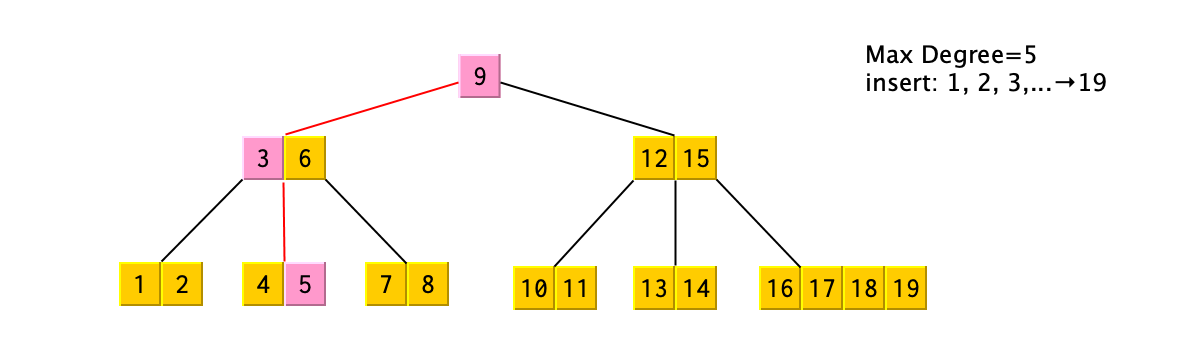
\includegraphics[keepaspectratio,alt={在Btree中查找''5''}]{images/Btree-order-5-search.png}}
\caption{在Btree中查找''5''}
\end{figure}

通常当\({\displaystyle M}\)较小时，我们在节点中查找的时候只需要进行顺序查找即可；如果较大的情况下，可以进行二分查找提高搜索的效率。

\begin{Shaded}
\begin{Highlighting}[]
\ConstantTok{B}\OperatorTok{{-}}\ConstantTok{TREE}\OperatorTok{{-}}\ConstantTok{SEARCH}\NormalTok{(x, k)}
\NormalTok{  i ← }\DecValTok{1}
  \ControlFlowTok{while}\NormalTok{ i ≤ n}\KeywordTok{[}\NormalTok{x}\KeywordTok{]} \ControlFlowTok{and}\NormalTok{ k ≥ key}\KeywordTok{[}\NormalTok{x, i}\KeywordTok{]}
    \ControlFlowTok{do}\NormalTok{ i ← i }\OperatorTok{+} \DecValTok{1}
  \ControlFlowTok{if}\NormalTok{ i ≤ n}\KeywordTok{[}\NormalTok{x}\KeywordTok{]} \ControlFlowTok{and}\NormalTok{ k }\OperatorTok{=}\NormalTok{ key}\KeywordTok{[}\NormalTok{x, i}\KeywordTok{]}
    \ControlFlowTok{then} \ControlFlowTok{return}\NormalTok{ (x, i)}
  \ControlFlowTok{if}\NormalTok{ leaf}\KeywordTok{[}\NormalTok{x}\KeywordTok{]}
    \ControlFlowTok{then} \ControlFlowTok{return} \ConstantTok{NIL}
    \ControlFlowTok{else}\NormalTok{ c }\OperatorTok{=} \ConstantTok{DISK}\OperatorTok{{-}}\ConstantTok{READ}\NormalTok{(c}\KeywordTok{[}\NormalTok{x, i}\KeywordTok{]}\NormalTok{)}
      \ControlFlowTok{return} \ConstantTok{B}\OperatorTok{{-}}\ConstantTok{TREE}\OperatorTok{{-}}\ConstantTok{SEARCH}\NormalTok{(c, k)}
\end{Highlighting}
\end{Shaded}

\subsection{insert操作}\label{insertux64cdux4f5c}

\subsubsection{节点的分裂}\label{ux8282ux70b9ux7684ux5206ux88c2}

在进行insert之前，需要考虑的就是，btree规定了一个节点中最大的child的数目，当一个节点中子节点的数目超过允许的最大值的时候，需要将节点拆分为两个。例如上面的例子，如果再插入20的话，如果直接插入则子元素已经超出了最大允许的数目：

\begin{figure}
\centering
\pandocbounded{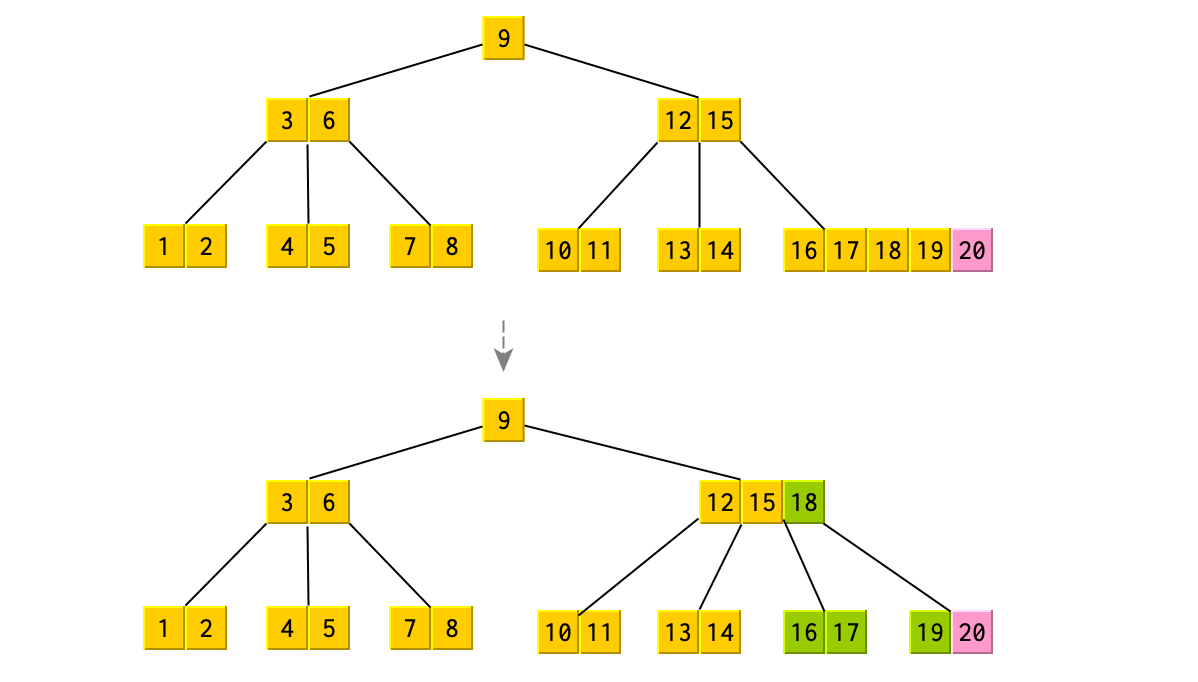
\includegraphics[keepaspectratio,alt={在Btree中插入''20''}]{images/Btree-order-5-split.png}}
\caption{在Btree中插入''20''}
\end{figure}

在上面的例子中，拆分之后，两个子节点的元素个数正好是平均的，但是，如果order为偶数的情况下是不平均的：

\begin{figure}
\centering
\pandocbounded{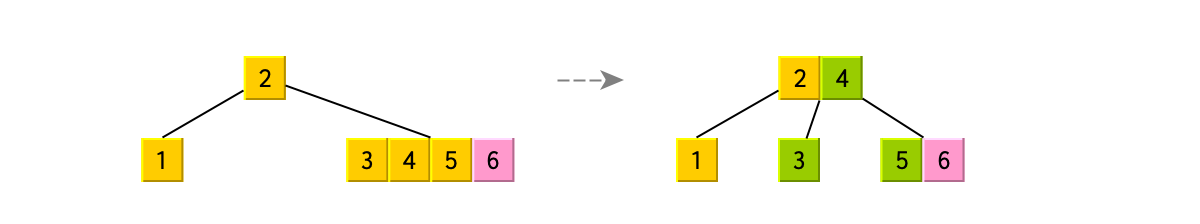
\includegraphics[keepaspectratio,alt={在Btree中插入''6''}]{images/Btree-order-4-split.png}}
\caption{在Btree中插入''6''}
\end{figure}

值得注意的是，因为每次分裂高度会增加，同时会增加父元素的key个数，那么也可能导致父节点满。所以如果上层节点也满了的话，也是需要递归的分裂的：

\begin{figure}
\centering
\pandocbounded{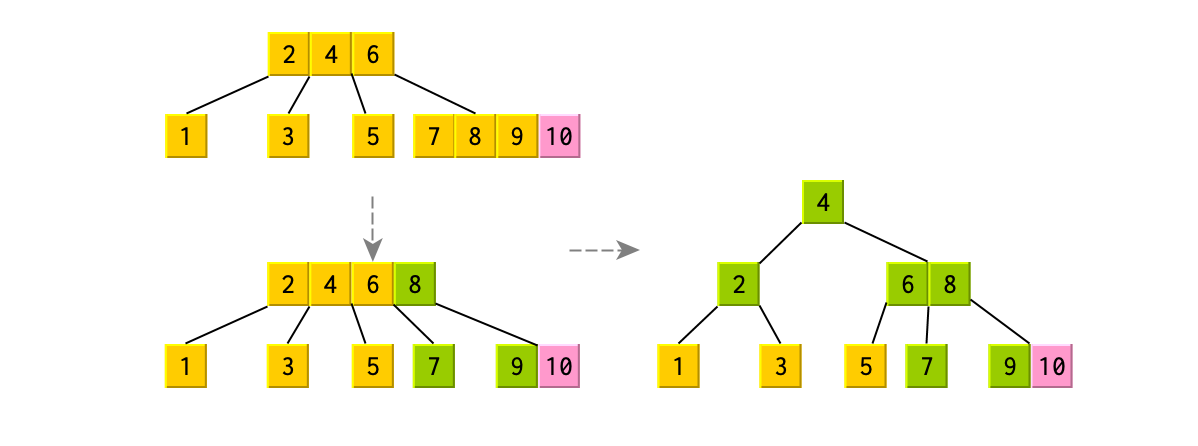
\includegraphics[keepaspectratio,alt={在Btree中插入''10''}]{images/Btree-order-4-multi-split.png}}
\caption{在Btree中插入''10''}
\end{figure}

\subsubsection{节点插入过程}\label{ux8282ux70b9ux63d2ux5165ux8fc7ux7a0b}

当order为奇数时，插入A\textasciitilde Q的过程如下：

\begin{figure}
\centering
\pandocbounded{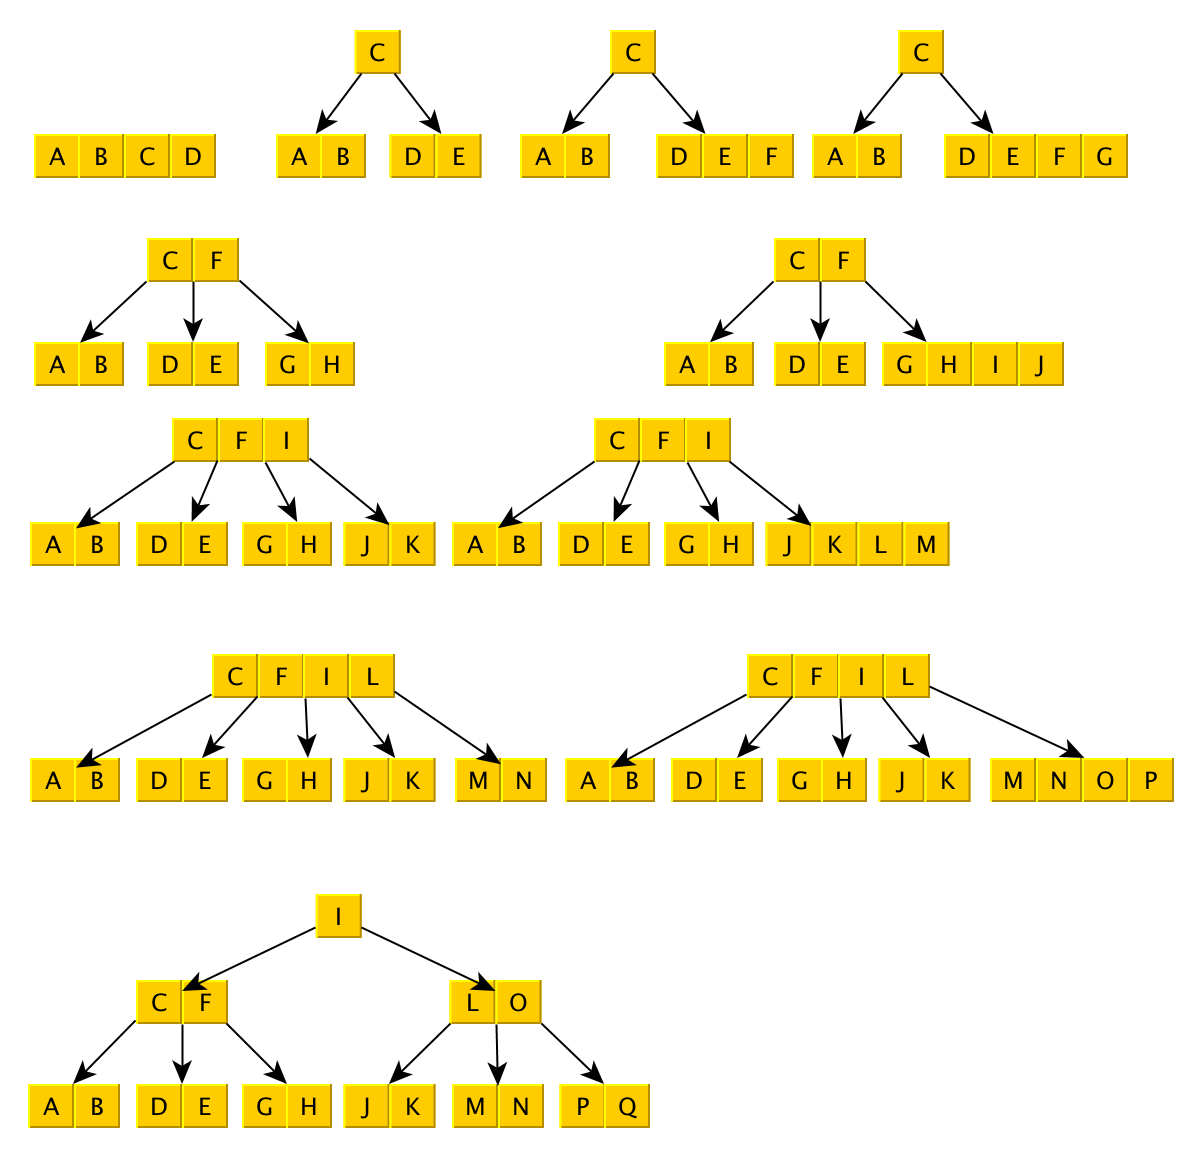
\includegraphics[keepaspectratio,alt={btree of order 5}]{images/btree_order_5_insert.png}}
\caption{btree of order 5}
\end{figure}

当order为偶数时，插入A-J的过程如下：

\begin{figure}
\centering
\pandocbounded{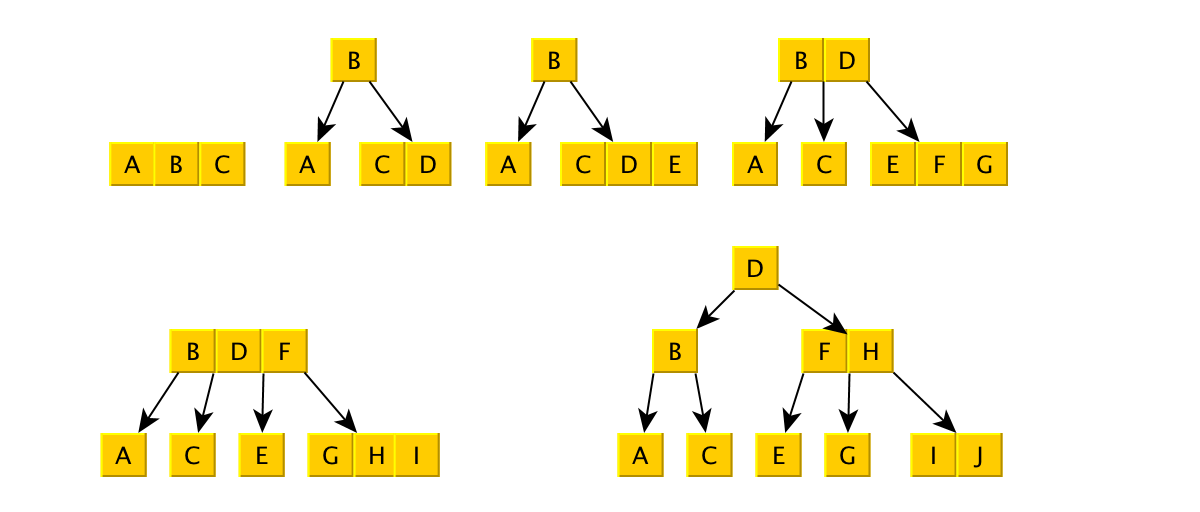
\includegraphics[keepaspectratio,alt={btree of order 4}]{images/btree_order_4_insert.png}}
\caption{btree of order 4}
\end{figure}

在Insert的过程中，一般的做法是先将元素插入到叶节点，这时候如果发现叶节点满了，需要将其Split，并将其中一个key提升到父节点中。同时，需要看父节点是否满，如果满了也需要进行拆分，直到根节点。但是这种做法需要插入后再回溯，比较难以实现。\href{http://staff.ustc.edu.cn/~csli/graduate/algorithms/book6/chap19.htm}{另一种方式}则是在插入的过程中，一旦发现节点已经满了，无法再容纳元素，则先将其拆分，然后再继续朝下查找。这样只需要查找一次，再最后插入到叶子节点的时候，能够保证不会溢出。

\subsubsection{抢占式分裂（Preemtive Split）}\label{ux62a2ux5360ux5f0fux5206ux88c2preemtive-split}

如上所说，在insert操作的时候，是先插入元素，然后再进行拆分的，这样可能插入之后还需要一直递归到上层节点进行拆分。例如下面的一个场景：

\begin{figure}
\centering
\pandocbounded{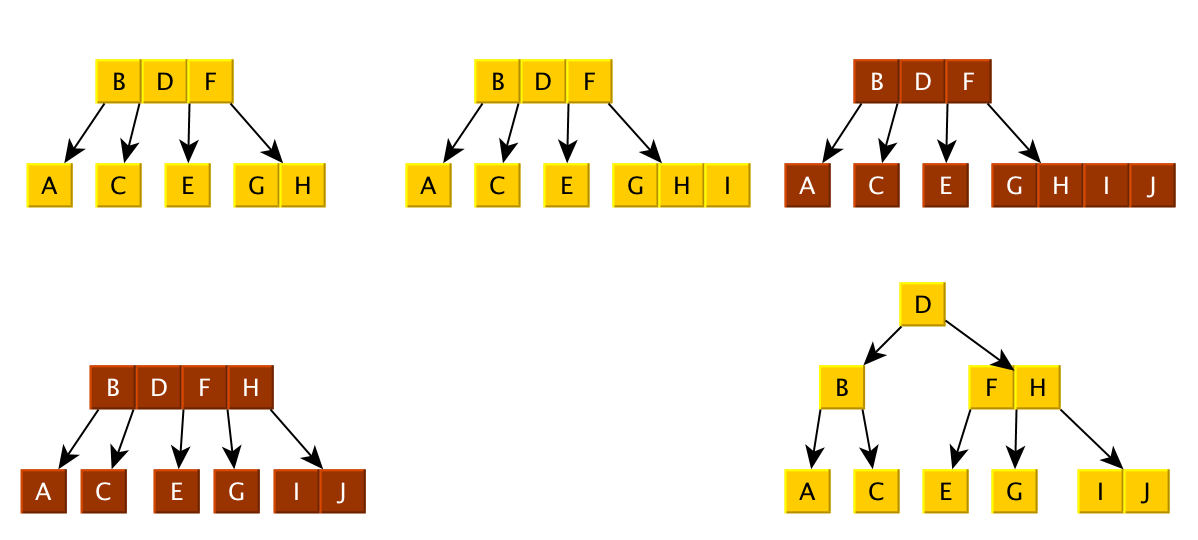
\includegraphics[keepaspectratio,alt={btree of order 4}]{images/btree_order_4_insert_normal.png}}
\caption{btree of order 4}
\end{figure}

而Preemtive Split正是在insert之前即进行拆分，当发现一个节点快要满了的时候，就先split之后再插入，自顶向下，不需要再回溯到上一层的节点。

\begin{figure}
\centering
\pandocbounded{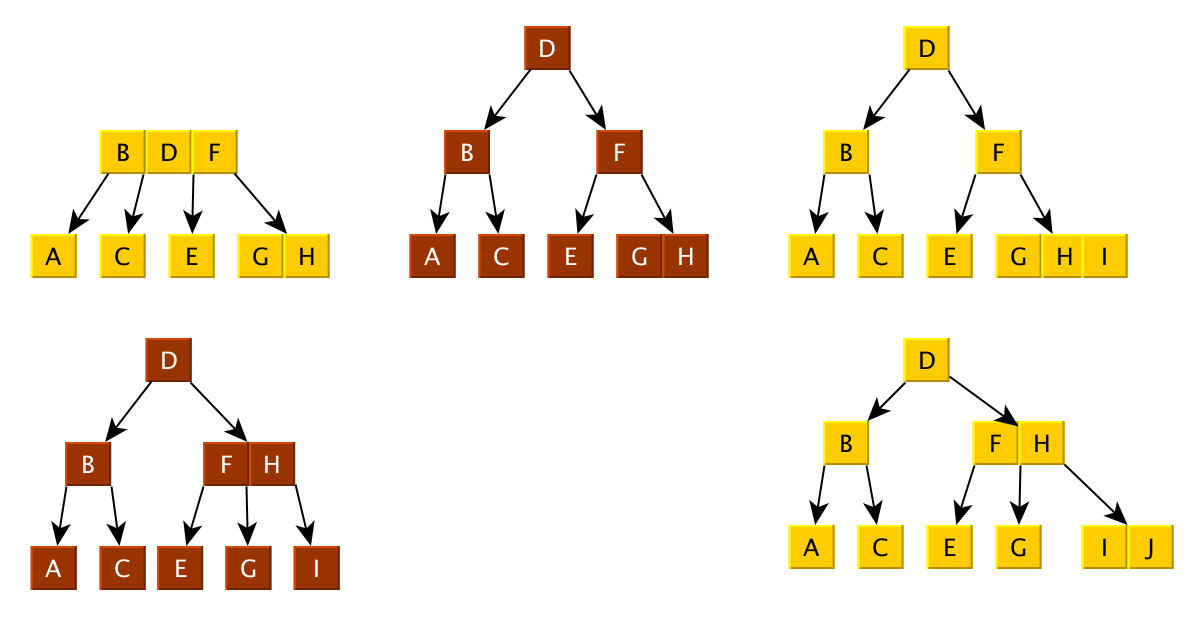
\includegraphics[keepaspectratio,alt={btree of order 4}]{images/btree_order_4_insert_preemtive.png}}
\caption{btree of order 4}
\end{figure}

从上面的例子可以看到，两种方式构造出的Btree在插入I之后其实是不大一样的，而当J插入之后则变成一致了。

\subsection{创建一个空的B-tree}\label{ux521bux5efaux4e00ux4e2aux7a7aux7684b-tree}

\begin{Shaded}
\begin{Highlighting}[]
\ConstantTok{B}\OperatorTok{{-}}\ConstantTok{TREE}\OperatorTok{{-}}\ConstantTok{CREATE}\NormalTok{(}\ConstantTok{T}\NormalTok{)}
\NormalTok{  x ← }\ConstantTok{ALLOCATE}\OperatorTok{{-}}\ConstantTok{NODE}\NormalTok{()}
\NormalTok{  leaf}\KeywordTok{[}\NormalTok{x}\KeywordTok{]}\NormalTok{ ← }\ConstantTok{TRUE}
\NormalTok{  n}\KeywordTok{[}\NormalTok{n}\KeywordTok{]}\NormalTok{ ← }\DecValTok{0}
  \ConstantTok{DISK}\OperatorTok{{-}}\ConstantTok{WRITE}\NormalTok{(x)}
\NormalTok{  root}\KeywordTok{[}\ConstantTok{T}\KeywordTok{]}\NormalTok{ ← x}
\end{Highlighting}
\end{Shaded}

\subsection{删除操作}\label{ux5220ux9664ux64cdux4f5c}

\section{B-Tree变种}\label{b-treeux53d8ux79cd}

\begin{itemize}
\tightlist
\item
  2-3-4树：Order为4的B-tree又被称之为2-3-4 tree (每个非叶子节点有2个、3个或者4个子节点)
\item
  2-3树：Order为3的B-tree又被称之为2-3 tree (每个非叶子节点有2个或者3个子节点)
\item
  B+-tree：A B-tree in which keys are stored in the leaves.
\item
  B*-tree：A B-tree in which nodes are kept 2/3 full by redistributing keys to fill two child nodes, then splitting them into three nodes.
\end{itemize}

参考资料:

\begin{itemize}
\tightlist
\item
  \href{https://en.wikipedia.org/wiki/B-tree}{Wikipedia - B-tree}
\item
  \href{https://www.cs.usfca.edu/~galles/cs673/lecture/lecture11.pdf}{Graduate Algorithms CS673-2016F-11 B-Trees}
\item
  \href{https://xlinux.nist.gov/dads/HTML/btree.html}{NIST B-tree}
\item
  \href{http://staff.ustc.edu.cn/~csli/graduate/algorithms/book6/chap19.htm}{CHAPTER 19: B-TREES}
\item
  \href{https://stackoverflow.com/questions/28846377/what-is-the-difference-btw-order-and-degree-in-terms-of-tree-data-structure}{What is the difference btw ``Order'' and ``Degree'' in terms of Tree data structure}
\end{itemize}


\end{document}
